% Options for packages loaded elsewhere
\PassOptionsToPackage{unicode}{hyperref}
\PassOptionsToPackage{hyphens}{url}
%
\documentclass[
]{article}
\usepackage{lmodern}
\usepackage{amssymb,amsmath}
\usepackage{ifxetex,ifluatex}
\ifnum 0\ifxetex 1\fi\ifluatex 1\fi=0 % if pdftex
  \usepackage[T1]{fontenc}
  \usepackage[utf8]{inputenc}
  \usepackage{textcomp} % provide euro and other symbols
\else % if luatex or xetex
  \usepackage{unicode-math}
  \defaultfontfeatures{Scale=MatchLowercase}
  \defaultfontfeatures[\rmfamily]{Ligatures=TeX,Scale=1}
\fi
% Use upquote if available, for straight quotes in verbatim environments
\IfFileExists{upquote.sty}{\usepackage{upquote}}{}
\IfFileExists{microtype.sty}{% use microtype if available
  \usepackage[]{microtype}
  \UseMicrotypeSet[protrusion]{basicmath} % disable protrusion for tt fonts
}{}
\makeatletter
\@ifundefined{KOMAClassName}{% if non-KOMA class
  \IfFileExists{parskip.sty}{%
    \usepackage{parskip}
  }{% else
    \setlength{\parindent}{0pt}
    \setlength{\parskip}{6pt plus 2pt minus 1pt}}
}{% if KOMA class
  \KOMAoptions{parskip=half}}
\makeatother
\usepackage{xcolor}
\IfFileExists{xurl.sty}{\usepackage{xurl}}{} % add URL line breaks if available
\IfFileExists{bookmark.sty}{\usepackage{bookmark}}{\usepackage{hyperref}}
\hypersetup{
  hidelinks,
  pdfcreator={LaTeX via pandoc}}
\urlstyle{same} % disable monospaced font for URLs
\usepackage[margin=1in]{geometry}
\usepackage{longtable,booktabs}
% Correct order of tables after \paragraph or \subparagraph
\usepackage{etoolbox}
\makeatletter
\patchcmd\longtable{\par}{\if@noskipsec\mbox{}\fi\par}{}{}
\makeatother
% Allow footnotes in longtable head/foot
\IfFileExists{footnotehyper.sty}{\usepackage{footnotehyper}}{\usepackage{footnote}}
\makesavenoteenv{longtable}
\usepackage{graphicx,grffile}
\makeatletter
\def\maxwidth{\ifdim\Gin@nat@width>\linewidth\linewidth\else\Gin@nat@width\fi}
\def\maxheight{\ifdim\Gin@nat@height>\textheight\textheight\else\Gin@nat@height\fi}
\makeatother
% Scale images if necessary, so that they will not overflow the page
% margins by default, and it is still possible to overwrite the defaults
% using explicit options in \includegraphics[width, height, ...]{}
\setkeys{Gin}{width=\maxwidth,height=\maxheight,keepaspectratio}
% Set default figure placement to htbp
\makeatletter
\def\fps@figure{htbp}
\makeatother
\setlength{\emergencystretch}{3em} % prevent overfull lines
\providecommand{\tightlist}{%
  \setlength{\itemsep}{0pt}\setlength{\parskip}{0pt}}
\setcounter{secnumdepth}{-\maxdimen} % remove section numbering
\usepackage{setspace}\doublespacing
\usepackage{lineno}\linenumbers

\author{}
\date{\vspace{-2.5em}}

\begin{document}

\textbf{Classification:} Biological Sciences -- Evolution \hfill\break

\begin{center}
\textbf{A Standardized Effect Size for Evaluating and Comparing the Strength of Phylogenetic Signal}
\end{center}

\hfill\break

\begin{center}
\textbf{Dean C. Adams$^{1 *}$, Erica K. Baken$^{1,2}$,  and Michael L. Collyer$^{2}$}
\end{center}

\hfill\break

\(^{1}\)Department of Ecology, Evolution, and Organismal Biology, Iowa
State University, Ames, Iowa, USA.

\(^{2}\)Department of Science, Chatham University, Pittsburgh,
Pennsylvania, USA.

\(^{*}\)Correspondence: Dean C. Adams. Department of Ecology, Evolution,
and Organismal Biology, Iowa State University, Ames, Iowa, USA.
515-294-3834.
\href{mailto:dcadams@iastate.edu}{\nolinkurl{dcadams@iastate.edu}}

\hfill\break

\begin{center}15 July, 2020\end{center}

\hfill\break

\begin{longtable}[]{@{}rr@{}}
\toprule
words & characters\tabularnewline
\midrule
\endhead
2553 & 16162\tabularnewline
\bottomrule
\end{longtable}

\newpage

\hypertarget{abstract}{%
\section{Abstract}\label{abstract}}

Macroevolutionary studies frequently characterize the phylogenetic
signal in phenotypes, and wish to compare the strength of that signal
across traits. However, analytical tools for such comparisons have
largely remained underdeveloped. Here we evaluate the efficacy of one
commonly used parameter (Pagel's \(\lambda\)) to estimate the strength
of phylogenetic signal in phenotypic traits, and evaluate the degree to
which \(\lambda\) correctly identifies known levels of phylogenetic
signal. We find that \(\lambda\) behaves as a Bernoulli random variable,
and that estimates are increasingly skewed at larger and smaller input
levels of phylogenetic signal. Further, the precision of \(\lambda\) in
estimating actual levels of phylogenetic signal is often inaccurate, and
biological interpretations of the strength of phylogenetic signal based
on \(\lambda\) are therefore compromised. We propose a standardized
effect size based on \(\kappa\), (\(Z_\kappa\)), which measures the
strength of phylogenetic signal more reliably than does \(\lambda\), and
places that signal on a common scale for statistical comparison. We
develop tests based on \(Z_\kappa\) to provide a mechanism for formally
comparing the strength of phylogenetic signal across datasets, in much
the same manner as effect sizes may be used to summarize patterns in
quantitative meta-analysis. Our approach extends the phylogenetic
comparative toolkit to address hypotheses that compare the strength of
phylogenetic signal between various phenotypic traits, even when those
traits are found in different evolutionary lineages or have different
units or scales. \hfill\break

\textbf{Keywords}: phylogenetic signal, macroevolution, lambda, kappa

\newpage

\hypertarget{significance-statement}{%
\section{Significance Statement}\label{significance-statement}}

Evolutionary biologists wish to quantify and compare the strength of
phylogenetic signal across traits, but analytical tools for these
comparisons are generally lacking. Here we develop a standardized effect
size based on \(\kappa\) (\(Z_\kappa\)), which measures the strength of
phylogenetic signal on a common statistical scale, and provides a
mechanism for formally comparing the strength of phylogenetic signal
across datasets. Additionally, we find that a commonly used parameter
(Pagel's \(\lambda\)) is insuitable for this purpose. Our procedure
enables biologists to quantitatively address hypotheses that compare the
strength of phylogenetic signal between various phenotypic traits, even
when those traits are found in different evolutionary lineages or have
different units or scales.

\newpage

\hypertarget{introduction}{%
\section{Introduction}\label{introduction}}

Investigating macroevolutionary patterns of trait variation requires a
phylogenetic perspective, because the shared ancestry among species
violates the assumption of independence among trait values that is
common for statistical tests (1, 2). Accounting for this evolutionary
non-independence is the purview of \emph{phylogenetic comparative
methods} (PCMs): a suite of analytical tools that condition trends in
the data on the phylogenetic relatedness of observations (3--12). These
methods are predicated on the notion that phylogenetic signal -- the
tendancy for closely related species to display similar trait values --
is present in cross-species datasets (1, 13, 14). Indeed, under numerous
evolutionary models, phylogenetic signal is to be expected, as
stochastic character change along the hierarchical structure of the tree
of life generates trait covaration among related taxa (1, 14, 15).
\hfill\break

Several analytical tools have been developed to quantify phylogenetic
signal in phenotypic datasets (13, 14, 16--19), and their statistical
properties -- namely type I error rates and statistical power -- have
been investigated to determine under what conditions phylogenetic signal
can be detected (15, 18, 20--25). One of the most widely used methods
for characterizing phylogenetic signal is Pagel's \(\lambda\) (13),
which transforms the lengths of the internal branches of the phylogeny
to improve the fit of data to the phylogeny via maximum likelihood (13,
26). When incorporated in PGLS, \(\lambda\) serves as a tuning parameter
(ranging from \(0\rightarrow1\)) which is optimized via log-likelihood
profiling while evaluating the covariation between the dependent and
independent variables, given the phylogeny (13, 26). To infer whether
phylogenetic signal differs from no signal or a Brownian motion model of
evolutionary divergence, the observed model fit using \(\hat\lambda\)
may be statistically compared to that using \(\lambda=0\) or
\(\lambda=1\) via likelihood ratio tests (26--28) or confidence limits
(29). Another widely used measure is Blomberg's \(\kappa\) (14), which
measures the ratio of observed trait variation to the amount expected
under Brownian motion. Blomberg's \(\kappa\) can be treated as a test
statistic by employing a permutation test to generate its sampling
distribution (14, 18) for determining whether significant phylogenetic
signal is present in data. Both \(\lambda\) and \(\kappa\) seem
intuitive to interpret, as a value of \(0\) for both corresponds to no
phylogenetic signal, while a value of \(1\) corresponds to the amount of
phylogenetic signal expected under Brownian motion. Thus, it is tempting
to regard both \(\lambda\) and \(\kappa\) as descriptive statistics that
measure the relative strength of phylogenetic signal, providing an
estimate of its magnitude for comparison. \hfill\break

The appeal of Pagel's \(\lambda\) and Blomberg's \(\kappa\) as
descriptive statistics is that they provide a basis for interpreting
``weak'' versus ``strong'' phylogenetic signal; i.e., small versus large
values of \(\hat{\lambda}\) or \(\kappa\), respectively, in a
comparative sense (30--32). Nonetheless, an important question that has
yet to be considered is whether these statistics are or can be converted
to effect sizes for comparative analyses across datasets? To be
statistics representing phylogenetic signal, they should have reliable
distributional properties, which could be revealed with simulation
experiments. For instance, as a proportional random variable bounded by
\(0\) and \(1\), we might expect that \(\hat{\lambda}\) follows a
Bernoulli distribution (\textbf{add ref}); i.e., branch lengths in a
tree are scaled proportionally to the probability that data arise from a
BM process. Given a known \(\lambda\) value used to generate random data
on a tree, we would also expect that the mean of an empirical sampling
distribution of \(\hat{\lambda}\) would approximately equal \(\lambda\);
the dispersion of \(\hat{\lambda}\) would be largest at intermediate
values of \(\lambda\), \(\hat{\lambda}\) would be predictable over the
range of \(\lambda\) with respect to treesize; the distribution of
\(\hat{\lambda}\) would be symmetric at intermediate values of
\(\lambda\) and more skewed toward values of 0 or 1; and that the
distribution of \(\hat{\lambda}\) will be more platykurtic at
intermediate values of \(\lambda\), becoming more leptokurtic toward 0
and 1 (\textbf{add same ref}). Prior work (20) seems to support some of
these conjectures, based superficially on statistical moments for a
given tree size (mean, variance, skewness, and kurtosis; see Fig. 2 of
(20)). However, because the ``strength of Brownian motion'' was
simulated as a varied weighted-average of data simulated on trees with
\(\lambda=0\) and \(\lambda=1\) and not prescribed values of \(\lambda\)
(20), interpretation of these patterns is challenging. \hfill\break

By contrast, Blomberg's \(\kappa\), which is positively ubounded, might
be expected to follow a normal distribution (\textbf{add ref}). Thus we
might expect that \(\kappa\) is symmetrically distributed across
different strengths of phylogenetic signal, for any \(\lambda\) used to
generate data. This attribute seemed less reasonable based on the
simulations performed by Münkemüller et al.~(20), as distibutions were
postively skewed, suggesting the Blomberg's \(\kappa\) might not behave
as a statistic that follows a noraml distribution. However, because
their simulations used a weighted combination of simulated phylogenetic
signal strengths, strong inferences are not possible (and distributional
attributes were not the intended result of their simulations). For both
Pagel's \(\lambda\) or Blomberg's \(\kappa\), evaluation of statistical
moments across a range of \(\lambda\) used to generate data would be
valuable for adjudicating the relibalilty of these statistics.
Furthermore, these are statistics that appear to have expected values
that vary with tree size (20), making comparisons across studies
challenging. Therefore, transformation of these statistics into
\(Z\)-scores in the same simulation experiments would allow evaluation
of the efficacy of each statistic to yield effect sizes that could be
used for comparative anlyses. \hfill\break

Here we used simulation experiments to compare the distributional
attributes of \(\hat{\lambda}\) and Blomberg's \(\kappa\), plus their
effect sizes (\(Z\)-scores), across a range of tree size and
phylogenetic signal strength. We find that estimates of
\(\hat{\lambda}\) are increasingly skewed at larger and smaller input
levels of phylogenetic signal, vary widely for a given input value of
\(\lambda\), and that the precision of \(\hat{\lambda}\) is not constant
across its range. By contrast, estimates of \(\kappa\) are more
consistent across tree sizes, and are normally distributed across the
range of input levels of \(\lambda\). We then propose an effect size
based on \(\kappa\) (\(Z_{\kappa}\)), which provides consistent
estimates of the strength of phylogenetic signal across tree sizes, and
facilitates quantitative comparisons of the relative strength of
phylogenetic signal across datasets.

\hypertarget{results}{%
\section{Results}\label{results}}

\textbf{Lambda (\(\lambda\)) estimates of phylogenetic signal are
innacurate.} Computer simulations revealed that for \(\hat{\lambda}\),
the distributional expectations of a Bernoulli variable were mostly
upheld. First, the mean value of \(\hat{\lambda}\) increased as
\(\lambda\) increased (Fig. 1 black line); the standard deviation of
\(\hat{\lambda}\) was largest at intermediate values of \(\lambda\) and
smallest at extreme values (Fig. 1 red line); and the distributions of
\(\hat{\lambda}\) were increasing skewed at extreme values of
\(\lambda\) but rather normal at intermediate values (Fig. 1 blue line).
For small tree sizes, it was also clear that distributions were more
platykurtik at intermeidate values of \(\hat{\lambda}\). Second,
\(\hat{\lambda}\) was a negatively-biased estimate of \(\lambda\) for
small tree sizes, as the mean value was consistently less than the input
\(\lambda\) value. Third, standard deviations of \(\hat{\lambda}\) were
negatively associated with tree size, and for tress of 128 species or
less, \(\hat{\lambda}\) was quite variable, except for cases when
\(\lambda\) was near or equal to \(1\). As such its statistical
properties make it insuitable as an effect size for measuring the
strength of phylogenetic signal. \hfill\break

\textbf{Kappa (\(\kappa\)) estimates of phylogenetic signal are more
stable.} Results for \(\kappa\) demonstrated better statistical
properties. First, mean values increased consistently with \(\lambda\)
irespective of tree size (Fig. 2 black line); the standard deviation of
\(\kappa\) was consistent across tree sizes (Fig. 2 red line); and
\(\kappa\) was normally distributed regardless of \(\lambda\) or tree
size (Fig. 2 blue line). The standard deviation of \(\kappa\) increased
with \(\lambda\), somewhat tracking the mean, but was always less than
the corresponding means. This is perhaps unsurprising, as \(\kappa\) is
bound by 0, and was never large for small values of \(\lambda\).
Finally, distributions of \(\kappa\) displayed slight skewing only at
small tree sizes and when \(\lambda\) was near or equal to 1. This
differs from the results of (20), where skewing appears to be from
combining random values generated independently. \hfill\break

\textbf{Effect sizes from \(\kappa\) (\(Z_{\kappa}\)) better
characterize phylogenetic signal.} We derived effect sizes (Z-scores)
for both \(\lambda\) and \(\kappa\) (see Methods) and evaluated them
relative to known phylogenetic signal. Both \(Z_{\lambda}\) and
\(Z_{\kappa}\) were associated with input phylogenetic signal
(\(\lambda\)), indicating that both statistics captured the observed
signal (Fig. 3). However, effect sizes from \(\hat{\lambda}\) made
little sense, as they were more strongly associated with tree size than
the actual phylogenetic signal in the data (Fig. 3). By contrast,
\(Z_{\kappa}\) was much more consistent accross tree sizes, and
exhibited a much stronger association with phylogenetic signal strength
as compared to tree size (Fig. 3). Thus between the two statistics,
\(Z_{\kappa}\) is a more reliable measure of the strength of
phylogenetic signal, and may be used to compare levels of phylogenetic
signal across datasets. \hfill\break

\textbf{A test statistic (\(\hat{Z}_{12}\)) allows meaningful
comparisons across datasets.} We derived a two-sample test statistic
(\(\hat{Z}_{12}\)) for statistically comparing the strength of
phylogenetic signal across datasets (see Methods). To demonstrate its
utility, we compared \(Z_{\kappa}\) for two ecologically-relevant traits
in plethodontid salamander (Fig. 4): surface area to volume ratios
(SA:V) and relative body width (\(\frac{BW}{SVL}\)) (33, 34). While both
contained significant phylogenetic signal, tests based on
\(\hat{Z}_{12}\) revealed that the degree of phylogenetic signal was
significantly stronger in SA:V (Fig. 4). Biologically, this observation
corresponds with the fact that tropical species -- which form a
monophyletic group within plethodontids -- display greater variation in
SA:V which covaries with disparity in their climatic niches (34).

\hypertarget{discussion}{%
\section{Discussion}\label{discussion}}

address hypotheses that compare the strength of phylogenetic signal
between various phenotypic traits, even when those traits are found in
different evolutionary lineages or have different units or scales

\hypertarget{methods}{%
\section{Methods}\label{methods}}

\textbf{Derivation of effect sizes.} Statistically, a standardized
effect size may be found as:

\begin{align}
    Z_{\theta}=\frac{\theta_{obs}-E(\theta)}{\sigma_\theta}
\end{align}

where \(\theta_{obs}\) is the observed test statistic, \(E(\theta)\) is
its expected value under the null hypothesis, and \(\sigma_\theta\) is
its standard error (35--37). Typically, \(\theta_{obs}\) and
\(\sigma_\theta\) are estimated from the data, while \(E(\theta)\) is
obtained from the distribution of \(\theta\) derived from parametric
theory. However, recent advances in resampling theory (38--41) have
shown that \(E(\theta)\) and \(\sigma_\theta\) may also be obtained from
an empirical sampling distribution of \(\theta\) obtained from
permutation procedures. \hfill\break

Formalizing the suggestion of Adams and Collyer (42), an effect size for
\(\kappa\) may be found as:

\begin{align}
    Z_\kappa=\frac{\kappa_{obs}-\hat\mu_{\kappa}}{\hat\sigma_{\kappa}},
\end{align}

where \(\kappa_{obs}\) is the observed phylogenetic signal, and
\(\hat\mu_\kappa\) and \(\hat\sigma_\kappa\) are the mean and standard
deviation of the empirical sampling distribution of \(\kappa\) obtained
via permutation. The empirical sampling distribution of \(\kappa\) is
first transformed via Box-Cox to better adhere to the assumption of
normality. \hfill\break

For \(\lambda\) deriving an effect size is more challenging, it does not
have a sampling distribution from which the standard error (and thus
confidence intervals) may be obtained. Thus, its confidence intervals
are generated for the values of \(\lambda\) that intersect the
log-likehihood profile for corresponding percentiles of the \(\chi^2\)
distribution used to compare the compare the putative appropriate model
to a null model with \(\lambda = 0\) {[}\textbf{add ref: MLC thinks
Boettiger paper?}{]}. As such, an effect size for \(\lambda\) may be
found as:

\begin{align}
   \lvert Z_{\lambda} \rvert = \sqrt{\chi^2_{\hat{\lambda}}}
\end{align}

where, \(\hat{\lambda}\) is the maximized likelihood value of
\(\lambda\) and \(\chi^{2}_{\hat{\lambda}}\) is the likelihood ratio
statistic for the value. Note that alternative formulations could be
envisioned: \(Z_{\lambda} = d \sqrt{\chi^2_{\hat{\lambda}}}\), where
\(d\) is a binary value \((-1,1)\) to indicate a direction based on
whether \(\hat{\lambda}\) is below or above a critical value of
\(\lambda\), for a quantile from a \(\chi^{2}\) distribution at a
probability of 0.5. However, preliminary investigations found that
mapping \(\chi^2_{\hat{\lambda}}\) values in this manner did not produce
effect sizes that were symmetrical about \(Z = 0\), as the mapping was
not linear and the log-likelihood profiles can be rather flat for small
trees. \hfill\break

\textbf{Derivation of two-sample test statistic.} To compare the
strength of phylogenetic signal across datasets, a two-sample test
statistic may be calculated as:

\begin{align}
  \hat{Z}_{12}=\frac{\lvert{(\kappa_{1}-\hat\mu_{\kappa_1})-(\kappa_{2}-\hat\mu_{\kappa_2})}\rvert}{\sqrt{\hat\sigma^2_{\kappa_1}+\hat\sigma^2_{\kappa_2}}} = \frac{\lvert Z_{\kappa_1} - Z_{\kappa_2}\rvert}{\sqrt{2}}
\end{align}

where \(\kappa_1\), \(\kappa_2\), \(\hat\mu_{\kappa_1}\),
\(\hat\mu_{\kappa_2}\), \(\hat\sigma_{\kappa_1}\), and
\(\hat\sigma_{\kappa_2}\) are as defined above for equation 2. The right
side of the equation illustrates that if \(Z_\kappa\) has already been
calculated for two sampling distributions as in equation 2, the sampling
distributions have unit variance for each of the \(Z_\kappa\)
statistics. Estimates of significance of \(\hat{Z}_{12}\) may be
obtained from a standard normal distribution. Typically,
\(\hat{Z}_{12}\) is considered a two-tailed test, however directional
(one-tailed) tests may be specified should the empirical situation
require it (39, 41). \hfill\break

\textbf{Simulations.} Simulations were conducted by generating
pure-birth phylogenies at each of six different tree sizes
(\(n=2^5, 2^6, \cdots, 2^{10}\)), and with differing levels of
phylognetic signal (\(\lambda=0.0, 0.5, \cdots, 1.0\)). We generated 100
random trees for each intersection of tree size and \(\lambda\). For
each \(\lambda\) within each tree size, continuous traits were then
simulated on each phylogeny under a BM model of evolution. For each set
of 100 trees we measured the mean values of \(\hat{\lambda}\) and
\(\kappa\), their standard deviation, and calculated the Shapiro-Wilk
\(W\) statistic as a departure from normality (symmetry). For the
latter, a value of \(1.0\) indicates normally distributed values, while
departures from \(1.0\) indicate skewness. Simulations were then
repeated for both bananced and pectinate trees, which yielded
qualitatively similar results (see Supporting Information). Trees
containing polytomies, and an evaluation of \(\hat{\lambda}\) from
models of linear regression and phylogenetic ANOVA, were also
investigated, and results were qualitatively similar to those reported
above (see Supporting Information). \hfill\break

\textbf{Empirical Data.} Surface area to volume ratios (SA:V) and
relative body width (\(\frac{BW}{SVL}\)) measures were obtained from
individuals of 305 species (2,781 and 3,371 respectively), from which
species means were obtained (33, 34). A time-dated molecular phylogeny
for the group (43) was then pruned to match the species in the
phenotypic dataset. The phylogenetic signal in each trait was then
characterized using \(\kappa\), which was converted to its effect size
(\(Z_\kappa\)) using \texttt{geomorph} 3.3.1 (44, 45).

\hypertarget{acknowledgements}{%
\section{Acknowledgements}\label{acknowledgements}}

This work was supported in part by NSF grant DBI-1902511 (to D.C.A.) and
DBI-1902694 (to M.L.C.).

\newpage

\hypertarget{references}{%
\section{References}\label{references}}

\setlength{\parindent}{-0.25in} \setlength{\leftskip}{0.25in}
\setlength{\parskip}{8pt} \noindent

\hypertarget{refs}{}
\leavevmode\hypertarget{ref-Felsenstein1985}{}%
1. J. Felsenstein, Phylogenies and the comparative method.
\emph{American Naturalist} \textbf{125}, 1--15 (1985).

\leavevmode\hypertarget{ref-HarveyPagel1991}{}%
2. P. H. Harvey, M. D. Pagel, \emph{The comparative method in
evolutionary biology} (Oxford University Press, 1991).

\leavevmode\hypertarget{ref-Grafen1989}{}%
3. A. Grafen, The phylogenetic regression. \emph{Philosophical
Transactions of the Royal Society of London B, Biological Sciences}
\textbf{326}, 119--157 (1989).

\leavevmode\hypertarget{ref-GarlandIves2000}{}%
4. T. J. Garland, A. R. Ives, Using the past to predict the present:
Confidence intervals for regression equations in phylogenetic
comparative methods. \emph{American Naturalist} \textbf{155}, 346--364
(2000).

\leavevmode\hypertarget{ref-Rohlf2001}{}%
5. F. J. Rohlf, Comparative methods for the analysis of continuous
variables: Geometric interpretations. \emph{Evolution} \textbf{55},
2143--2160 (2001).

\leavevmode\hypertarget{ref-ButlerKing2004}{}%
6. M. A. Butler, A. A. King, Phylogenetic comparative analysis: A
modeling approach for adaptive evolution. \emph{American Naturalist}
\textbf{164}, 683--695 (2004).

\leavevmode\hypertarget{ref-MartinsHansen1997}{}%
7. E. P. Martins, T. F. Hansen, Phylogenies and the comparative method:
A general approach to incorporating phylogenetic information into the
analysis of interspecific data. \emph{American Naturalist} \textbf{149},
646--667 (1997).

\leavevmode\hypertarget{ref-OMeara_et_al2006}{}%
8. B. C. O'Meara, C. Ane, M. J. Sanderson, P. C. Wainwright, Testing for
different rates of continuous trait evolution using likelihood.
\emph{Evolution} \textbf{60}, 922--933 (2006).

\leavevmode\hypertarget{ref-RevellHarmon2008}{}%
9. L. J. Revell, L. J. Harmon, Testing quantitative genetic hypotheses
about the evolutionary rate matrix for continuous characters.
\emph{Evolutionary Ecology Research} \textbf{10}, 311--331 (2008).

\leavevmode\hypertarget{ref-Beaulieu_et_al2012}{}%
10. J. M. Beaulieu, D. C. Jhwueng, C. Boettiger, B. C. O'Meara, Modeling
stabilizing selection: Expanding the ornstein-uhlenbeck model of
adaptive evolution. \emph{Evolution} \textbf{66}, 2369--2383 (2012).

\leavevmode\hypertarget{ref-Adams2014b}{}%
11. D. C. Adams, A method for assessing phylogenetic least squares
models for shape and other high-dimensional multivariate data.
\emph{Evolution} \textbf{68}, 2675--2688 (2014).

\leavevmode\hypertarget{ref-AdamsCollyer2018b}{}%
12. D. C. Adams, M. L. Collyer, Phylogenetic anova: Group-clade
aggregation, biological challenges, and a refined permutation procedure.
\emph{Evolution} \textbf{72}, 1204--1215 (2018).

\leavevmode\hypertarget{ref-Pagel1999}{}%
13. M. D. Pagel, Inferring the historical patterns of biological
evolution. \emph{Nature} \textbf{401}, 877--884 (1999).

\leavevmode\hypertarget{ref-Blomberg_et_al2003}{}%
14. S. P. Blomberg, T. Garland, A. R. Ives, Testing for phylogenetic
signal in comparative data: Behavioral traits are more labile.
\emph{Evolution} \textbf{57}, 717--745 (2003).

\leavevmode\hypertarget{ref-Revell_et_al2008}{}%
15. L. J. Revell, L. J. Harmon, D. C. Collar, Phylogenetic signal,
evolutionary process, and rate. \emph{Systematic Biology} \textbf{57},
591--601 (2008).

\leavevmode\hypertarget{ref-Abouheif1999}{}%
16. E. Abouheif, A method for testing the assumption of phylogenetic
independence in comparative data. \emph{Evolutionary Ecology Research}
\textbf{1}, 895--909 (1999).

\leavevmode\hypertarget{ref-Gittleman1990}{}%
17. J. L. Gittleman, M. Kot, Adaptation: Statistics and a null model for
estimating phylogenetic effects. \emph{Systematic Zoology} \textbf{39},
227--241 (1990).

\leavevmode\hypertarget{ref-Adams2014a}{}%
18. D. C. Adams, A generalized Kappa statistic for estimating
phylogenetic signal from shape and other high-dimensional dultivariate
data. \emph{Systematic Biology} \textbf{63}, 685--697 (2014).

\leavevmode\hypertarget{ref-Klingenberg2010}{}%
19. C. P. Klingenberg, N. A. Gidaszewski, Testing and quantifying
phylogenetic signals and homoplasy in morphometric data.
\emph{Systematic biology} \textbf{59}, 245--261 (2010).

\leavevmode\hypertarget{ref-Munkemuller_et_al2012}{}%
20. T. Münkemüller\emph{et al.}, How to measure and test phylogenetic
signal. \emph{Methods in Ecology and Evolution} \textbf{3}, 743--756
(2012).

\leavevmode\hypertarget{ref-Pavoine2012}{}%
21. S. Pavoine, C. Ricotta, Testing for phylogenetic signal in
biological traits: The ubiquity of cross-product statistics.
\emph{Evolution: International Journal of Organic Evolution}
\textbf{67}, 828--840 (2012).

\leavevmode\hypertarget{ref-DinizFilho2012}{}%
22. J. A. F. Diniz-Filho, T. Santos, T. F. Rangel, L. M. Bini, A
comparison of metrics for estimating phylogenetic signal under
alternative evolutionary models. \emph{Genetics and Molecular Biology}
\textbf{35}, 673--679 (2012).

\leavevmode\hypertarget{ref-MolinaVenegas2017}{}%
23. R. Molina-Venegas, M. A. Rodríguez, Revisiting phylogenetic signal;
strong or negligible impacts of polytomies and branch length
information? \emph{BMC evolutionary biology} \textbf{17}, 53 (2017).

\leavevmode\hypertarget{ref-Revell2010}{}%
24. L. J. Revell, Phylogenetic signal and linear regression on species
data. \emph{Methods in Ecology and Evolution} \textbf{1}, 319--329
(2010).

\leavevmode\hypertarget{ref-Boettiger_et_al2012}{}%
25. C. Boettiger, G. Coop, P. Ralph, Is your phylogeny informative?
Measuring the power of comparative methods. \emph{Evolution}
\textbf{67}, 2240--2251 (2012).

\leavevmode\hypertarget{ref-Freckleton_et_al2002}{}%
26. R. P. Freckleton, P. H. Harvey, M. Pagel, Phylogenetic analysis and
comparative data: A test and review of evidence. \emph{American
Naturalist} \textbf{160}, 712--726 (2002).

\leavevmode\hypertarget{ref-Cooper2010}{}%
27. N. Cooper, W. Jetz, R. P. Freckleton, Phylogenetic comparative
approaches for studying niche conservatism. \emph{Journal of
Evolutionary Biology} \textbf{23}, 2529--2539 (2010).

\leavevmode\hypertarget{ref-Bose2019}{}%
28. R. Bose, B. R. Ramesh, R. Pélissier, F. Munoz, Phylogenetic
diversity in the western ghats biodiversity hotspot reflects
environmental filtering and past niche diversification of trees.
\emph{Journal of Biogeography} \textbf{46}, 145--157 (2019).

\leavevmode\hypertarget{ref-Vandelook2019}{}%
29. F. Vandelook\emph{et al.}, Nectar traits differ between pollination
syndromes in balsaminaceae. \emph{Annals of Botany} \textbf{124},
269--279 (2019).

\leavevmode\hypertarget{ref-DeMeester2019}{}%
30. G. De Meester, K. Huyghe, R. Van Damme, Brain size, ecology and
sociality: A reptilian perspective. \emph{Biological Journal of the
Linnean Society} \textbf{126}, 381--391 (2019).

\leavevmode\hypertarget{ref-Pintanel2019}{}%
31. P. Pintanel, M. Tejedo, S. R. Ron, G. A. Llorente, A. Merino-Viteri,
Elevational and microclimatic drivers of thermal tolerance in andean
pristimantis frogs. \emph{Journal of Biogeography} \textbf{46},
1664--1675 (2019).

\leavevmode\hypertarget{ref-Su2019}{}%
32. G. Su, S. Villéger, S. Brosse, Morphological diversity of freshwater
fishes differs between realms, but morphologically extreme species are
widespread. \emph{Global ecology and biogeography} \textbf{28}, 211--221
(2019).

\leavevmode\hypertarget{ref-Baken2019}{}%
33. E. K. Baken, D. C. Adams, Macroevolution of arboreality in
salamanders. \emph{Ecology and Evolution} \textbf{9}, 7005--7016 (2019).

\leavevmode\hypertarget{ref-Baken2020}{}%
34. E. K. Baken, L. E. Mellenthin, D. C. Adams, Macroevolution of
desiccation‐related morphology in plethodontid salamanders as inferred
from a novel surface area to volume ratio estimation approach.
\emph{Evolution} \textbf{74}, 476--486 (2020).

\leavevmode\hypertarget{ref-Glass1976}{}%
35. G. V. Glass, Primary, secondary, and meta-analysis of research.
\emph{Educational Researcher} \textbf{5}, 3--8 (1976).

\leavevmode\hypertarget{ref-Cohen1988}{}%
36. J. Cohen, \emph{Statistical power analysis for the behavioral
sciences} (Routledge, 1988).

\leavevmode\hypertarget{ref-Rosenthal1994}{}%
37. R. Rosenthal, ``The handbook of research synthesis'' in L. V. Cooper
H Hedges, Ed. (Russell Sage Foundation, 1994), pp. 231--244.

\leavevmode\hypertarget{ref-Collyer_et_al2015a}{}%
38. M. L. Collyer, D. J. Sekora, D. C. Adams, A method for analysis of
phenotypic change for phenotypes described by high-dimensional data.
\emph{Heredity} \textbf{115}, 357--365 (2015).

\leavevmode\hypertarget{ref-AdamsCollyer2016}{}%
39. D. C. Adams, M. L. Collyer, On the comparison of the strength of
morphological integration across morphometric datasets. \emph{Evolution}
\textbf{70}, 2623--2631 (2016).

\leavevmode\hypertarget{ref-CollyerAdams2018}{}%
40. M. L. Collyer, D. C. Adams, RRPP: An r package for fitting linear
models to high-dimensional data using residual randomization.
\emph{Methods in Ecology and Evolution} \textbf{9}, 1772--1779 (2018).

\leavevmode\hypertarget{ref-AdamsCollyer2019b}{}%
41. D. C. Adams, M. L. Collyer, Comparing the strength of modular
signal, and evaluating alternative modular hypotheses, using covariance
ratio effect sizes with morphometric data. \emph{Evolution} \textbf{73},
2352--2367 (2019).

\leavevmode\hypertarget{ref-AdamsCollyer2019}{}%
42. D. C. Adams, M. L. Collyer, Phylogenetic comparative methods and the
evolution of multivariate phenotypes. \emph{Annual Review of Ecology,
Evolution, and Systematics} \textbf{50}, 405--425 (2019).

\leavevmode\hypertarget{ref-Bonett2017}{}%
43. R. M. Bonett, A. L. Blair, Evidence for complex life cycle
constraints on salamander body form diversification. \emph{Proceedings
of the National Academy of Sciences, U.S.A.} \textbf{114}, 9936--9941
(2017).

\leavevmode\hypertarget{ref-AdamsOtarola2013}{}%
44. D. C. Adams, E. Otárola-Castillo, Geomorph: An r package for the
collection and analysis of geometric morphometric shape data.
\emph{Methods in Ecology and Evolution} \textbf{4}, 393--399 (2013).

\leavevmode\hypertarget{ref-AdamsGeomorph}{}%
45. D. C. Adams, M. L. Collyer, A. Kaliontzopoulou, Geomorph: Software
for geometric morphometric analyses. R package version 3.3.1. (2020).

\newpage

Real figures will have 6 panels for lambda and kappa and probably only a
subset for z. Simulations need to be re-run.

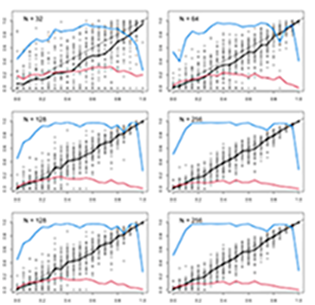
\includegraphics[width=0.95\linewidth]{new.fig.1.temp}

\singlespacing \textbf{Figure 1}. Temporary Fig. 1 showing lambda
patterns

\newpage

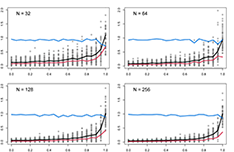
\includegraphics[width=0.95\linewidth]{new.fig.2.temp}

\singlespacing \textbf{Figure 2}. Temporary Fig. 2 showing kappa
patterns

\newpage

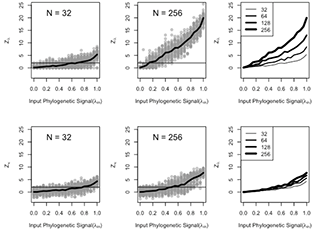
\includegraphics[width=0.95\linewidth]{new.fig.3.temp}

\singlespacing \textbf{Figure 3}. Temporary Fig. 3 showing z patterns

\newpage

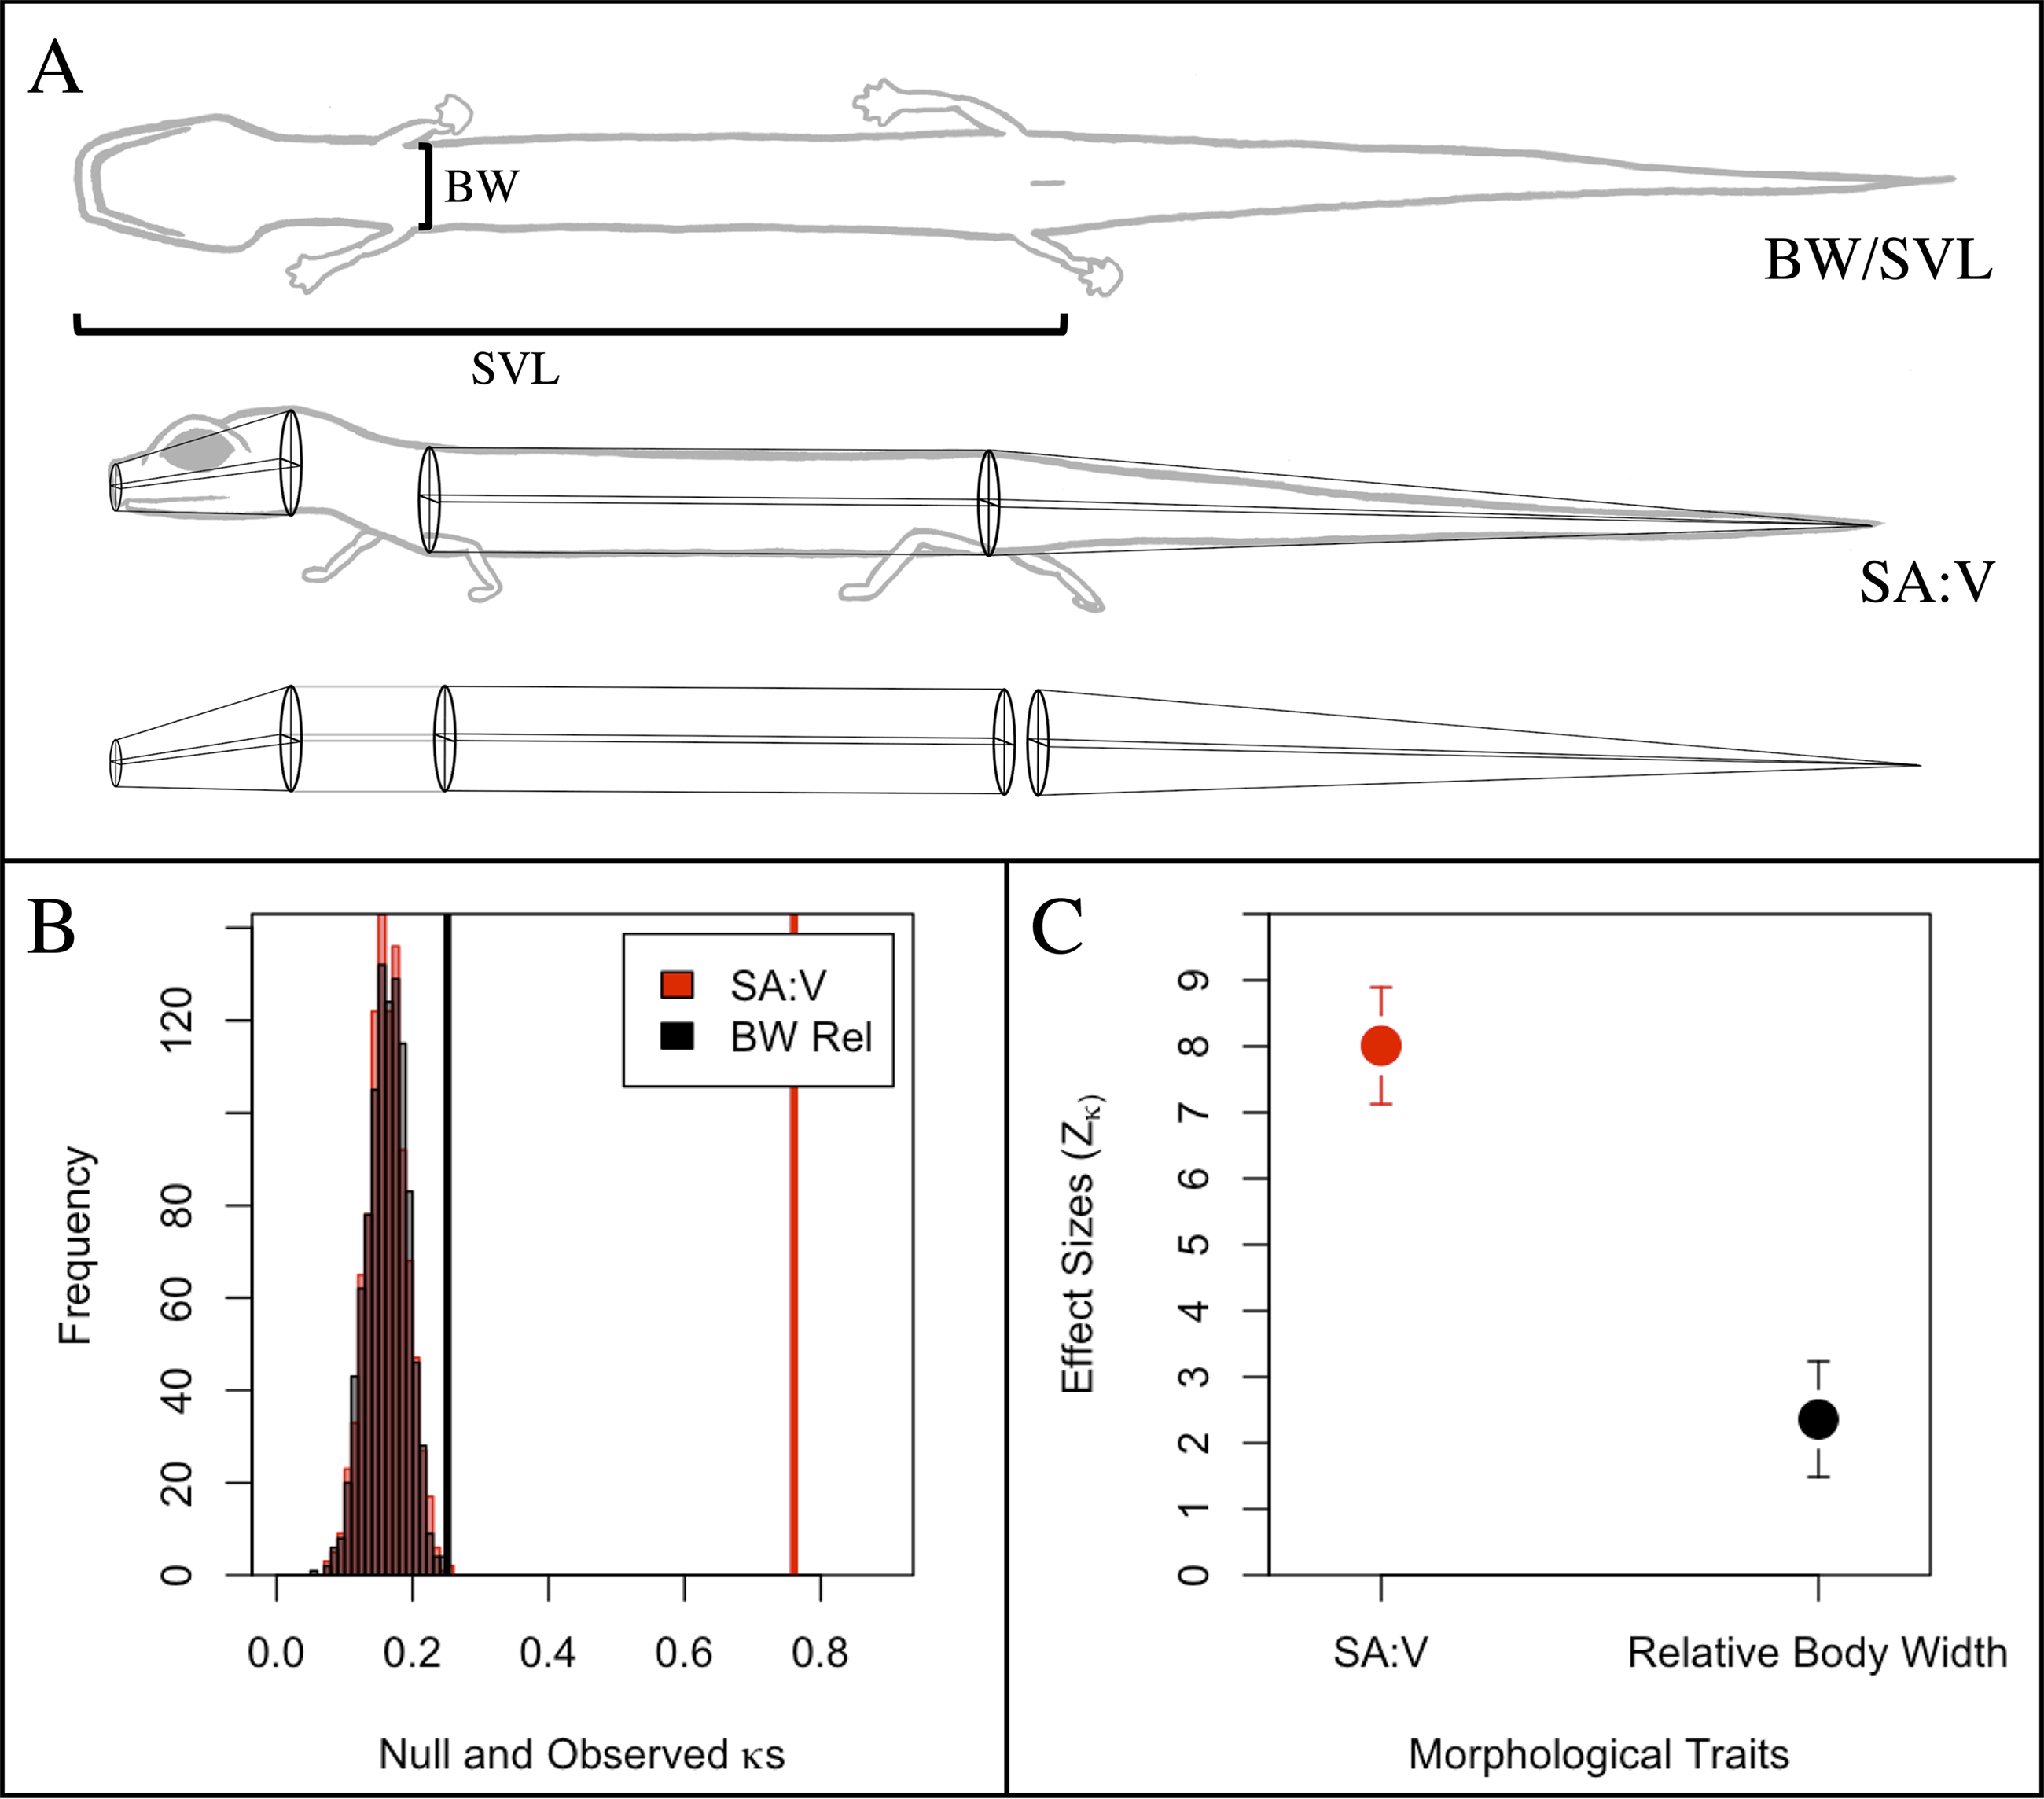
\includegraphics[width=0.95\linewidth]{new.fig.4}

\singlespacing \textbf{Figure 4}. (A) Linear measures for relative body
size, and regions of the body used to estimate surface area to volume
(SA:V) ratios. (B) Permutation distributions of phylogenetic signal for
SA:V and \(\frac{BW}{SVL}\), with observed values shown as vertical
bars. (C) Effect sizes (\(Z_\kappa\)) for SA:V and \(\frac{BW}{SVL}\),
with their 95\% confidence intervals (CI not standardized by
\(\sqrt(n)\)).

\end{document}
